\documentclass[9pt, technote, onecolumn]{IEEEtran}
\usepackage{graphicx}


\begin{document}

\title{Homework 2}
\author{Emma Fountain}
\maketitle

\section{Introduction}

I ran all experiments on the MSU HPCC from dev node "intel16", but using the job scheduler to actually run the experiments.

To compile the code I unzipped the repo using the \texttt{unzip} utility, navigated to the main folder, and ran \texttt{make}.

To run the code I set up a few basic utility scripts. First, I created \texttt{experiment.sh} wwhich runs the edge detection on each image 10 times, returning their average real runtime for each image. I used this file throughout the homework, modifying it slightly to point to different executables for different versions of the code. 

In addition I wrote a simple sbatch file which simply requested resources and ran this bash file.

All of the benchmarked times are given in Table I or Figure 1 on the following page.

\section{Serial Optimizations}

I first tried 4 different levels of compiler optimizations: \texttt{-O1, -O2, -O3} and \texttt{-Ofast}. As shown in the figure below, all of these performed significantly better than no optimization, but among the different levels there was not much of a difference except for the largest image, \texttt{earth.png}, which \texttt{-Ofast} performed slightly better on.

\centering
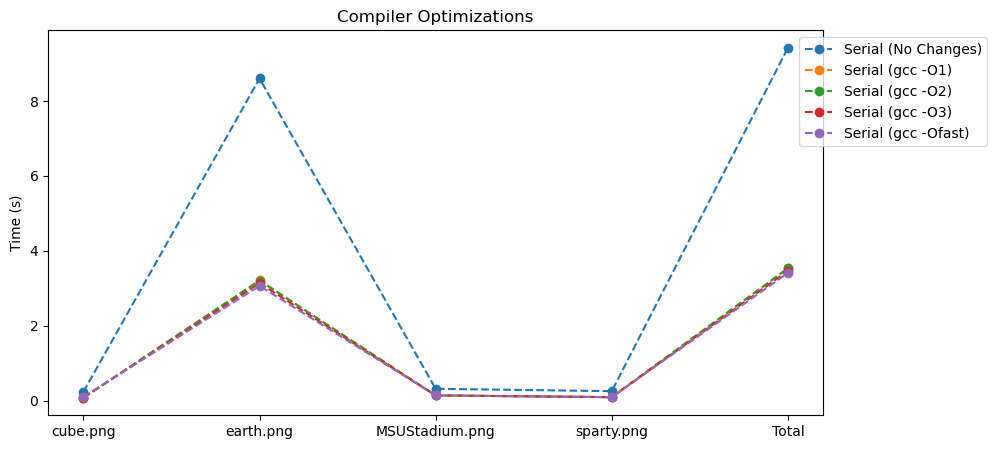
\includegraphics[width=6in]{CompilerOptimizations.png}

Next I tried inverting several loops. Many of these attempts actully raised the runtime, but inverting both the external nested loop and internal nested loop of the gradient calculation, for some reason, slightly improved the runtime as shown in the figure below.

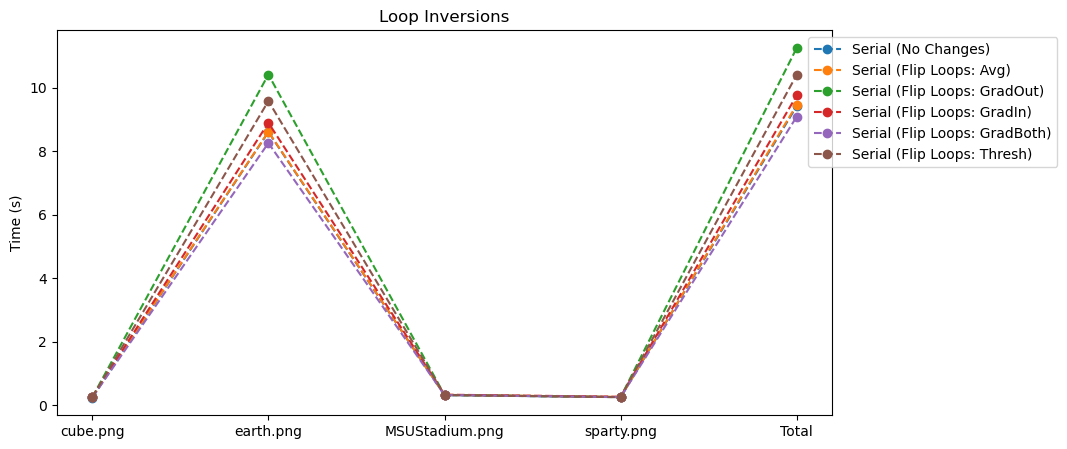
\includegraphics[width=6in]{LoopInversions.png}

The figure below shows a comparison between all serial versions of the code, including a version combining the 2 best optimizations I found; \texttt{-Ofast} and inverting both nested loops in the gradient calculation.

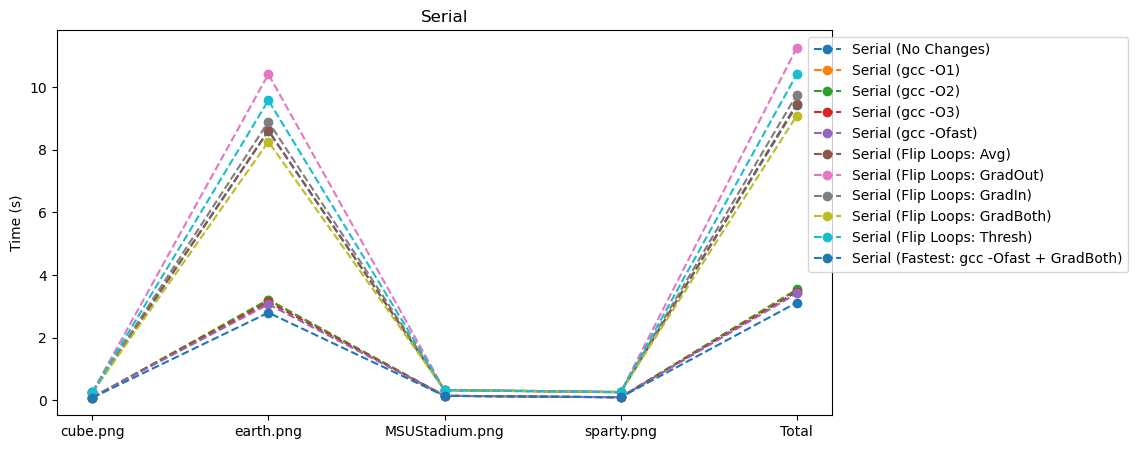
\includegraphics[width=6in]{Serial.png}

\section{OpenMP Optimization}

I parallelized the code by adding \texttt{\#pragma omp parallel for} directives in front of the loops for all 3 main steps. I chose to use 16 threads, and acheived a significant improvement over the best of the serial programs. In addition, I compiled this parallel version using the \texttt{-Ofast} compiler optimization which further increased the speed as shown in the figure below.

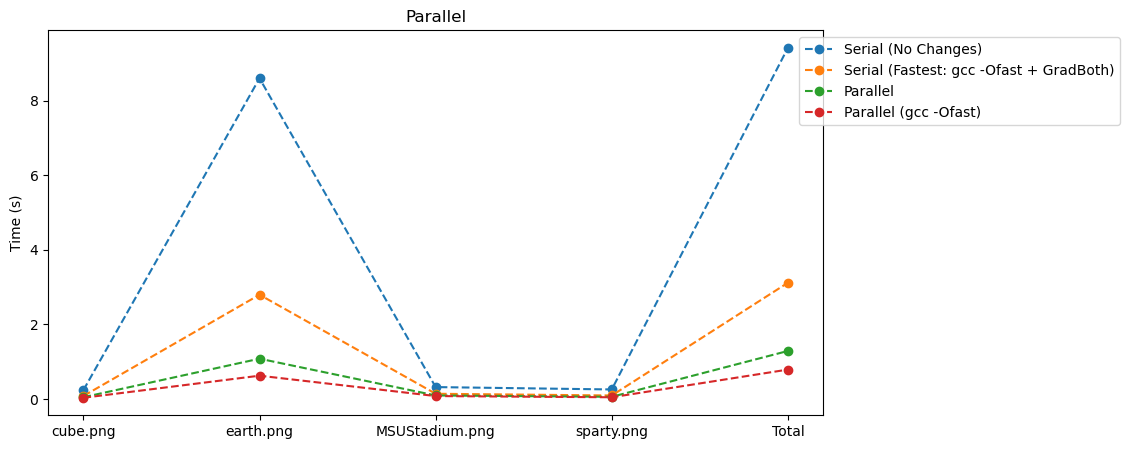
\includegraphics[width=6in]{Parallel.png}

\section{Conclusion}

This report shows that there are many ways to decrease runtime depending on your needs. Simply changing your compilation flags can significantly improve performance with essentially no additional work while for more demanding jobs it can be incredibly rewarding in terms of runtime to convert your code to run in parallel.

\newpage

\begin{figure*}
\centering
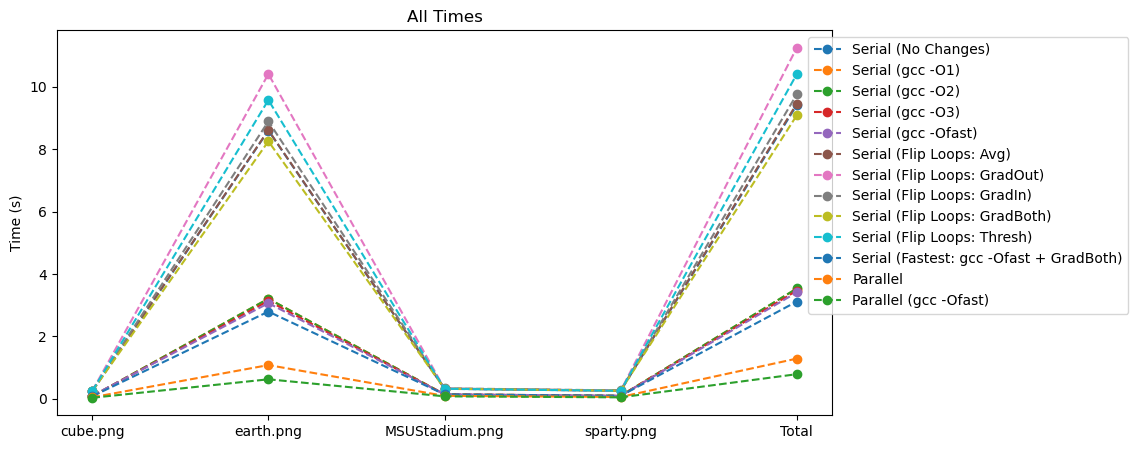
\includegraphics[width=6in]{AllTimes.png}
\caption{This figure shows times for all tests performed. Note the distinct clusters corresponding with different techniques such as serial compiler optimizations, loop inversions, and parallelization.}
\end{figure*}

\begin{table*}
    \renewcommand{\arraystretch}{1.3}
    \caption{Runtimes (Real)}
    \centering

    \begin{tabular}{|l||c|c|c|c|}
    \hline
    & \texttt{cube.png} & \texttt{earth.png} & \texttt{MSUStadium.png} & \texttt{sparty.png} \\ \hline
    \hline
	Serial (No Changes) &  0.2386 & 8.6005 & 0.3214 & 0.2578 \\ \hline \hline
	\hline
	Serial (gcc -O1) & 0.0816 & 3.2103 & 0.1428 & 0.0968 \\ \hline 
	Serial (gcc -O2) & 0.0842 & 3.210 & 0.1448 & 0.0986 \\ \hline 
	Serial (gcc -O3) & 0.0856 & 3.1397 & 0.145 & 0.0980 \\ \hline 
	Serial (gcc -Ofast) & 0.1033 & 3.067 & 0.1449 & 0.0978 \\ \hline 
	\hline
	Serial (Flip Loops: Avg) & 0.2549 & 8.612 & 0.3303 & 0.2651 \\ \hline 
	Serial (Flip Loops: GradOut) & 0.2548 & 10.4104 & 0.3272 & 0.2594 \\ \hline 
	Serial (Flip Loops: GradIn) & 0.2563 & 8.8933 & 0.3367 & 0.2708 \\ \hline 
	Serial (Flip Loops: GradBoth) & 0.2478 & 8.2549 & 0.3253 & 0.2606 \\ \hline 
	Serial (Flip Loops: Thresh) & 0.2504 & 9.5756 & 0.3238 & 0.257 \\ \hline 
	\hline
	Serial (Fastest: gcc -Ofast + GradBoth) & 0.0826 & 2.7977 & 0.1426 & 0.0961 \\ \hline 
	\hline
	Parallel & 0.0496 & 1.0827 & 0.0968 & 0.061 \\ \hline 
	Parallel (gcc -Ofast) & 0.0348 & 0.6269 & 0.0809 & 0.0483 \\ \hline 
    \end{tabular}

\end{table*}
\end{document}

